%%%%%%%%%%%%%%%%%%%%%%%%%%%%%%%%%%%%%%%%%%%%%%%%%%%%%%%%%%%%%%%%%%%%%%%
%                                                                     %
%             Sample document to demonstrate the class.               %
%                                                                     %
%%%%%%%%%%%%%%%%%%%%%%%%%%%%%%%%%%%%%%%%%%%%%%%%%%%%%%%%%%%%%%%%%%%%%%%

\documentclass[slanted]{acmeyatcl} % default: \em~\slshape \emph~\textsl
% \documentclass[italics]{acmeyatcl} % \em~\itshape \emph~\textit

\usepackage[T1]      {fontenc}
\usepackage[utf8]    {inputenc}
\usepackage[english] {babel}

\usepackage{booktabs, tikz}
\usepackage[math]{blindtext}


%%%%%%%%%%%%%%%%%%%%%%%%%%%%%%%%%%%%%%%%%%%%%%%%%%%%%%%%%%%%%%%%%%%%%%%%%%%%%

\firstline{Wonderful journal}
\secondline{Extraordinary cool organization}
\thirdline{42/42/4242 at Lovely place}
\logo{%
  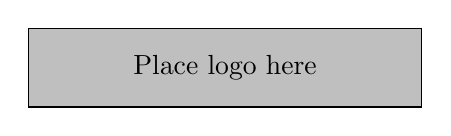
\begin{tikzpicture}
    \node [draw, fill=lightgray, minimum height=1cm, minimum width=5cm]
      {Place logo here};
  \end{tikzpicture}}


\begin{document}


\title{Lorem ipsum dolor sit amet, consectetur adipisicing}
\author{John Doe}

\email{John.Doe@domain.com}
\laboratory{Best lab in the world}
\affiliation{Best employer ever}
\moreinfos{Anything you want to add can go here.}


\maketitle

\nocite{lorem, ipsum}


\begin{abstract}
  \blindtext
\end{abstract}


\begin{twocols}

\Blinddocument

\end{twocols}


\section*{Figures}

\begin{twocols}

  \begin{figure}[H]
    \centering
    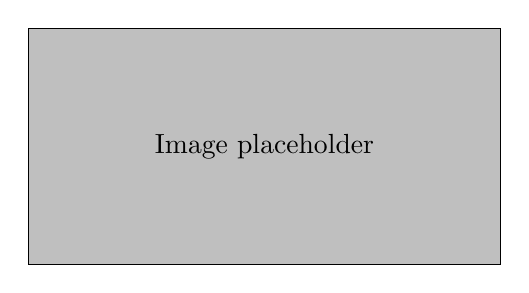
\begin{tikzpicture}
      \node [draw, fill=lightgray, minimum height=3cm, minimum width=6cm]
        {Image placeholder};
    \end{tikzpicture}
    \caption{Sample figure~1.}
  \end{figure}

  \begin{figure}[H]
    \centering
    
\begin{tikzpicture}
      \node [draw, fill=lightgray, minimum height=6cm, minimum width=5cm]
        {Image placeholder};
    \end{tikzpicture}
    \caption{Sample figure~2.}
  \end{figure}

\end{twocols}


\section*{Tables}

\begin{table}[H]
  \centering
  \begin{tabular}{rcl}
    \toprule
      \bfseries Right aligned &
      \bfseries Centered &
      \bfseries Left aligned \\
    \midrule
      1\up{st} cell & 2\up{nd} cell & 3\up{rd} and wide cell \\
      4\up{th} cell & 5\up{th} cell & 6\up{th} cell \\
      7\up{th} cell & 8\up{th} cell & 9\up{th} cell \\
    \bottomrule
  \end{tabular}
  \caption{Sample table.}
\end{table}


\bibliography{demo}


\end{document}
